% !TEX root = _individual/introduction.tex

%%%%%%%%%%%%%%%%%%%%%%%%%%%%%%%%%%%%%%%%%%%%%%%%%%%%%%%%%%%%%%%%%%%%%%%%%%%%%%%%
\chapter{Introduction}\label{chap:introduction}
%%%%%%%%%%%%%%%%%%%%%%%%%%%%%%%%%%%%%%%%%%%%%%%%%%%%%%%%%%%%%%%%%%%%%%%%%%%%%%%%

This thesis extends a steady-state, infinite-medium anisotropic diffusion (AD)
approximation \cite{Mor2007,Lar2009c} using a systematic derivation from the
transport equation that accounts for time-dependent behavior and arbitrary
problem boundaries. Our motivation is to formulate and test an approximation to
thermal radiative transfer (TRT) that is more accurate than diffusion yet much
less expensive than a time-dependent transport calculation.

%%%%%%%%%%%%%%%%%%%%%%%%%%%%%%%%%%%%%%%%%%%%%%%%%%%%%%%%%%%%%%%%%%%%%%%%%%%%%%%%
\section{Thermal radiative transfer}


Thermal radiative transfer is the dominant form of energy transfer in very
hot systems, such as the interior of a star or the target of a laser fusion
experiment. The equations that describe TRT not only have a large solution
phase space but also are strongly nonlinear; thus, they are difficult to solve
accurately and quickly.

%%%%%%%%%%%%%%%%%%%%%%%%%%%%%%%%%%%%%%%%%%%%%%%%%%%%%%%%%%%%%%%%%%%%%%%%%%%%%%%%
\section{Historical overview}

The past fifty years in which computers have been used to simulate radiative
transfer problems \cite{Cam1964,Cam1969} have seen unbelievable
advancements in computer technology.
Yet even today, with the need for increasingly accurate simulation of
increasingly
large and complex problems, computational power is still a limiting factor.
This is especially true in the burgeoning field of uncertainty quantification
(UQ), where large numbers of computer simulations are needed to gauge the
accuracy of the solution of a single problem.

It is one such problem in particular that inspired this work. The Center for
Radiative Shock Hydrodynamics (CRASH) program \cite{Crash2010} has the goal of
computationally predicting the behavior of a laser-driven shock in a
xenon-filled tube and providing ``error bars'' for that prediction. The accurate
simulation of energy traveling down a hollow pipe, via the process of
radiative transfer, is critical to modeling that problem. Several of the
numerical test problems in this thesis are based loosely on the CRASH problem.

Existing approximations to TRT, represented qualitatively in
Fig.~\ref{fig:fidelity}, are essentially either very accurate or very fast. On
the one hand are the full transport methods: Fleck and Cummings' Implicit Monte
Carlo (IMC) method \cite{Fle1971} and the discrete ordinates (\SN) method
\cite{Ada1998a}, both of which require significant time and large amounts of
computer memory. On the other hand are such coarse approximations as the
flux-limited diffusion (FLD) method \cite{Ols2000}, which makes a severe
approximation to the transport equation that yields a set of relatively simple
low-order equations. By developing a
time-dependent anisotropic diffusion approximation, we hope to provide a
\emph{via media} where a mild increase in run time is exchanged for a
significant increase in
accuracy. The AD method could then be applied to the CRASH project, or many
other TRT problems, to yield
realistic results in a realistic amount of time.

\begin{figure}[htb]
  \centering
  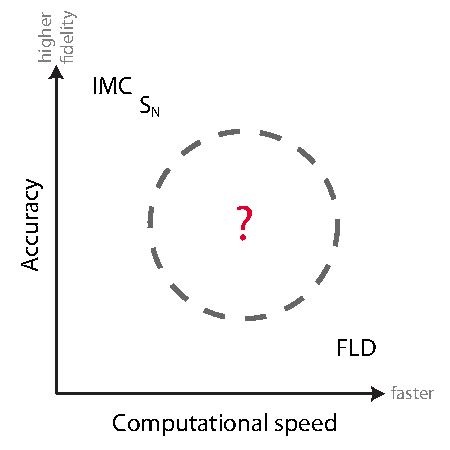
\includegraphics[width=3in]{fidelity}
  \caption{Figurative representation of existing TRT methods, showing the
  trade-off between accuracy and speed.}
  \label{fig:fidelity}
\end{figure}

%%%%%%%%%%%%%%%%%%%%%%%%%%%%%%%%%%%%%%%%%%%%%%%%%%%%%%%%%%%%%%%%%%%%%%%%%%%%%%%%
\section{Radiative transfer and anisotropic diffusion}
We begin by making some approximations to the radiative transfer
process that are common in methods development. By
\textsl{(i)} averaging over energy to get a ``gray'' (monoenergetic) radiation
intensity,
\textsl{(ii)} assuming that the material is at local thermodynamic equilibrium,
and
\textsl{(iii)} neglecting material conduction and advection,
we get a time-dependent radiation transport equation coupled to a single
material energy equation. The coupling process is the nonlinear Planckian
absorption and isotropic emission of photons: the hotter a material, the more
photons it emits.  Because the ``opacity'' of the material---%
the probability of a photon being absorbed during its flight---%
also depends on material temperature, colder materials tend to be more opaque,
or optically thick. The evolution of a system through time tends to show the
problem equilibrating by the progressive deposition of energy within a few mean
free paths of a hot region.

The anisotropic diffusion derivation starts by considering the radiation
transport equation over a time step. Rather than
making the simple diffusion approximation that the radiation intensity $I$ is a
linear function of angle, we use an integral transport equation in a novel way.
By making certain assumptions about how slowly the solution changes in space
and time, we can approximate the integral equation's nonlocal unknowns
with local unknowns. Massaging the result gives a set of low-order tensor
diffusion equations, where the AD tensor is calculated from a simple transport
equation that falls out of the analysis. Because the AD method retains a more
complicated representation of the radiation's angular behavior, we expect it
to give more accurate answers over a wide range of problems, especially those
where diffusion fails.

%Previous work \cite{Lar2009c} with the AD approximation showed very promising
%results in a steady-state Very High Temperature Reactor (VHTR) simulation;
%qualitatively, it showed how the anisotropic diffusion tensor allows particles
%to preferentially diffuse along a voided channel rather than acro

%%%%%%%%%%%%%%%%%%%%%%%%%%%%%%%%%%%%%%%%%%%%%%%%%%%%%%%%%%%%%%%%%%%%%%%%%%%%%%%%
\section{Contribution of this work}

%%%%%%%%%%%%%%%%%%%%%%%%%%%%%%%%%%%%%%%%%%%%%%%%%%%%%%%%%%%%%%%%%%%%%%%%%%%%%%%%
\section{Numerical experiments}

Derivation is only a part of developing a new method: it is also
crucial to run realistic numerical experiments that help determine the method's
efficiency and efficacy. This necessitates implementing not only the new method
but also its competitors. We have implemented
diffusion, FLD, \Pone, \SN, and IMC in the \pytrt\ code \cite{Pytrt}, freely
available to the public.

As mentioned, the phase space for TRT is very large: the radiation intensity
$I$ is a function of space $\vec{x}$, angle $\vec{\Omega}$, and time $t$;
the material temperature $T(\vec{x},t)$ is also a time- and space-dependent
quantity. Recently, a fictional ``flatland'' geometry has been successfully
used as a test
bed for new methods \cite{Lar2009c,Joh2011,Tra2011}. By restricting the travel
of particles to a two-dimensional plane, one angular variable is eliminated,
yet the complexity of multi-dimensional transport is retained. The
reduced solution phase space corresponds to a reduction in computer run time:
for Monte Carlo transport, the same number of particles yields a smaller
variance in the solution, and the \SN\ method requires fewer ordinates in the
quadrature set. Thus, we use flatland geometry for the majority of our test
problems.
Our extensive use of flatland has brought to light some
interesting peculiarities of the geometry \cite{Joh2011a}; these ancillary
results are presented in this thesis.

In addition to flatland problems, we also look at the performance of the AD
method in one-dimensional and two-dimensional problems seen in the
literature. These give insight into how well AD performs in a wider variety of
situations.

%%%%%%%%%%%%%%%%%%%%%%%%%%%%%%%%%%%%%%%%%%%%%%%%%%%%%%%%%%%%%%%%%%%%%%%%%%%%%%%%
\section{Synopsis}

The remainder of this thesis is organized into the following chapters.

\chaptersynopsis{chap:trtBackground}
The assertions about the difficulty of computational modelling of thermal
radiative transfer are bolstered by presenting the equations themselves. We give
a brief overview of existing approximations to the TRT equations and discuss how
those approximations are used in our work. Particular emphasis is given to the
semi-implicit treatment, which allows the nonlinear problem to be approximated
by a system of linear equations.

\chaptersynopsis{chap:adDerivation}
With the transport equation in hand, we derive a new approximation to radiation
transport, anisotropic diffusion. The derivation accounts for both time
dependence and boundary conditions. We then discuss some of the properties of
the AD method and make predictions for its range of applicability.

\chaptersynopsis{chap:aponeDerivation}
The derivation for the time-dependent AD equations assumed that the solution
changes very slowly in time, which can be a poor approximation when applied to
TRT: it can lead to the nonphysical transfer of energy faster than the speed of
light. This chapter addresses that shortcoming in two very different ways. The
first is to apply the physically motivated but \emph{ad hoc} method of flux
limiting to the AD formulation. The second is to modify the ansatz used in
deriving the anisotropic diffusion equations, leading to a new ``anisotropic
\Pone'' method.

\chaptersynopsis{chap:implementation}
The leakage terms for anisotropic diffusion are more complex than standard
diffusion: rather than a scalar diffusion coefficient, AD has a diffusion
tensor. This necessitates unusual discretization schemes in all but the simplest
of problems. We present new discretization schemes for Cartesian \xy\ geometry
that can account for the transverse leakage induced by the anisotropic diffusion
tensor.

\chaptersynopsis{chap:flatland}
As mentioned earlier, the ``flatland'' geometry has recently proven to be a
valuable test bed for new transport methods because of its smaller phase space
and correspondingly easier solution. This chapter gives a thorough overview of
the differences between flatland and true 3-D geometries, with a focus on
implementing flatland solvers. We also explore diffusion in flatland, not only
deriving the prior result that the diffusion coefficient is different but also
formulating correct diffusion boundary conditions. Finally, we present the AD
equations in flatland geometry.

\chaptersynopsis{chap:simpleNumericalResults}
Before applying the anisotropic approximations to full nonlinear transport in
multi-dimensional geometries, it is important that we test individual components
of the derivation. We detail several steady-state problems that test the
discretization schemes, flatland diffusion boundary conditions, and anisotropic
diffusion boundary conditions.

\chaptersynopsis{chap:trtNumericalResults}
Finally, we test the applicability of the anisotropic methods to the nonlinear
TRT equations. To begin, we look at a few simple 1-D test problems, where the
anisotropic methods merely ``smear'' the diffusion coefficients spatially. Then
we move to more complicated flatland problems that simulate radiation flow
through an optically thin channel, most applicable to the CRASH program.
Additionally, we apply the AD method to some difficult 2-D problems in the
literature that feature optically thick obstacles rather than optically thin
streaming channels.

\chaptersynopsis{chap:conclusion}
The final chapter summarizes the results of the theory developed in this thesis
and its application to TRT problems. We discuss possible improvements to the new
methods and other future work.

